\section{Regressionsanalyse}

Der zweite Teil der Arbeit beschäftigt sich mit der Regressionsanalyse.
Während die zuvor behandelte Korrelation nur die Stärke eines Zusammenhangs zwischen Merkmalen feststellt, ist es mittels der Regression möglich, auch die Richtung eines Zusammenhangs zu untersuchen.
Die Regression versucht dazu, die Werte eines abhängigen Merkmals mittels einer Funktion von den Werten eines unabhängigen Merkmals (Regressand) abzuleiten.


Die {\it NAG C Library} bietet dazu zahlreiche Funktionen, von verschiedenen Regressionsarten bis hin zu Hilfen für die Bewertung und Validierung von Regressionsmodellen.
%TODO: Kurze Einleitung erweitern
In der nächsten Sektion wird zunächst die einfache Regression vorgestellt, welche sich mit der Abhängigkeit eines Merkmals von einem Regressanden beschäftigt.
Für die theoretischen Grundlagen wurden \cite{Cramer2007} und \cite{Fahrmeir2010} zusammen mit der Einführung zur {\it NAG C Library} (\cite{nag:intro}) verwendet.

\subsection{Einfache Regression}

Wie bereits zuvor erwähnt existiert bei Anwendung der einfachen Regression immer nur ein Regressand.
Dennoch reicht diese einfache Form schon für viele Anwendungen aus, zum Beispiel wenn wir die Höhe der Mietpreise ($M$) in Abhängigkeit von der Wohnfläche ($W$) betrachten (vgl. \refsec{Anwendungsbeispiel}).
In diesem Falle ist der Mietpreis das abhängige Merkmal und die Wohnfläche der Regressand und beide sind metrisch skaliert.
Der allgemeine Ansatz zur Regression lautet somit:
\begin{equation*}
 M = f(W) + \epsilon
\end{equation*}
wobei die $f$ eine beliebige Funktion und $\epsilon$ ein Fehlerterm ist.
Dieser wird benötigt, da die den Merkmalen zugehörigen Datensätze $(m_1, \dots, m_n)$, bzw. $(w_1, \dots, w_n)$ nie \textit{genau} auf der Regressionsgeraden liegen, sondern durch Messfehler oder nicht berücksichtigte Abhängigkeiten abweichen.

Für Miete und Wohnfläche ist ein linearer Zusammenhang naheliegend.


\begin{itemize}
 \item Nichtlineare Regression
 \begin{itemize}
  \item Für Sättigungskurven und Wachstumsverläufe
  \item Mögliche Funktionen: exp, $x^2$, sin
  \item Berechnung durch kleinste Quadrate Methode mittels Transformation möglich
 \end{itemize}

 \item Beispiel: Regression der Nettomiete nach Wohnfläche
 \begin{itemize}
  \item Streudiagramm zeigt steigende Abweichung $\Rightarrow$ Multiple Regression nötig!
 \end{itemize}
\end{itemize}

\subsubsection{Beispiel}

\subsubsection{Anwendung}

\subsection{Multiple Regression}

Für den die Berechnung über Matrizen wird \cite{Fahrmeir1984} für die theoretischen Grundlagen verwendet.

Die multiple Regression ist zunächst einmal eine Erweiterung der einfachen Regression auf eine beliebige Anzahl von Regressoren.

\begin{equation}
  Y_i = \beta_0 + \beta_1 x_{i1} + \dots + \beta_p x_{ip} + \epsilon_i, \quad i = 1, \dots, n
\end{equation}
%TODO: Gleichung und Variablen erklären



\subsubsection{NAG Algorithmus}

In der NAG-Bibliothek wird die multiple Regression hauptsächlich durch die Funktion ... zur Verfügung gestellt.
%TODO: Welche anderen Funktionen sind noch beteiligt und was tuen diese?
 
%TODO: Ist eine alternative Strukturierung möglich, sodass weitere Unterkategorien wie QR-Zerlegung möglich sind?

\begin{equation}
  \label{eq:minimization}
  \sum\limits^{N}_{n=1} \epsilon^2_n = \epsilon^T \epsilon = (y - X \beta)^T (y - X \beta) \rightarrow \min\limits_{\beta}
\end{equation}


\begin{equation}
  \label{eq:minimization_general}
  \Vert X\beta - y \Vert_2 \rightarrow \min\limits_{\beta}
\end{equation}

\begin{equation}
  \label{eq:orthogonal_transformation}
  \Vert X\beta - y \Vert_2 = \Vert Q^T X \beta - Q^T y \Vert_2 = \Vert R \beta - c \Vert_2 + \Vert d \Vert_2
\end{equation}

\begin{figure}[t]
  \centering
  \begin{narrow}{-0.2\textwidth}{0.2\textwidth}
    \subfloat[][Subfloat 1]{
      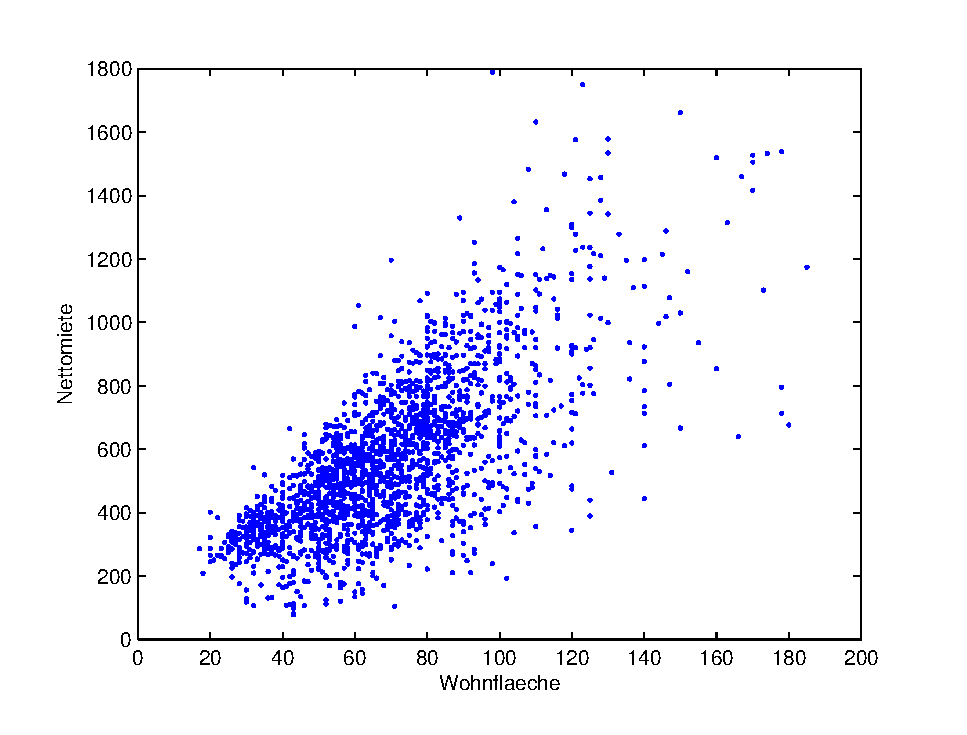
\includegraphics[width=0.7\textwidth]{figures/nm_wfl_distribution}
      \label{fig:nm_wfl_distributions:normal}
    }
    \subfloat[][Subfloat 2]{
      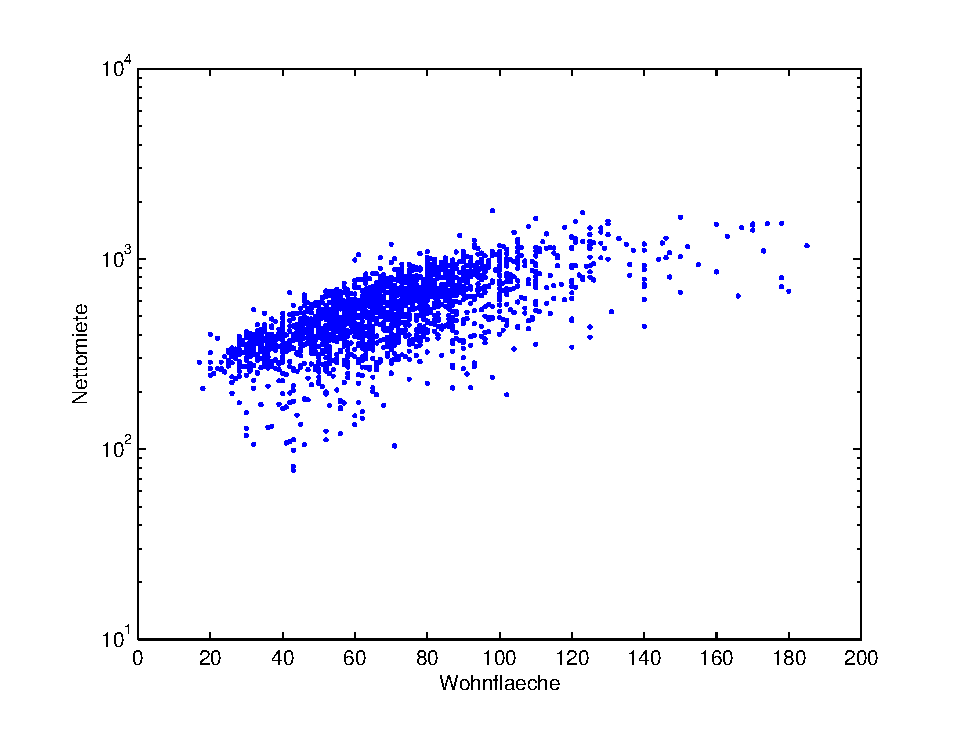
\includegraphics[width=0.7\textwidth]{figures/nm_wfl_distribution_log}
      \label{fig:nm_wfl_distributions:log}
    }
    \caption{Global caption}
  \end{narrow}
  \label{fig:nm_wfl_distributions}
\end{figure}

\begin{figure}[t]
  \centering
  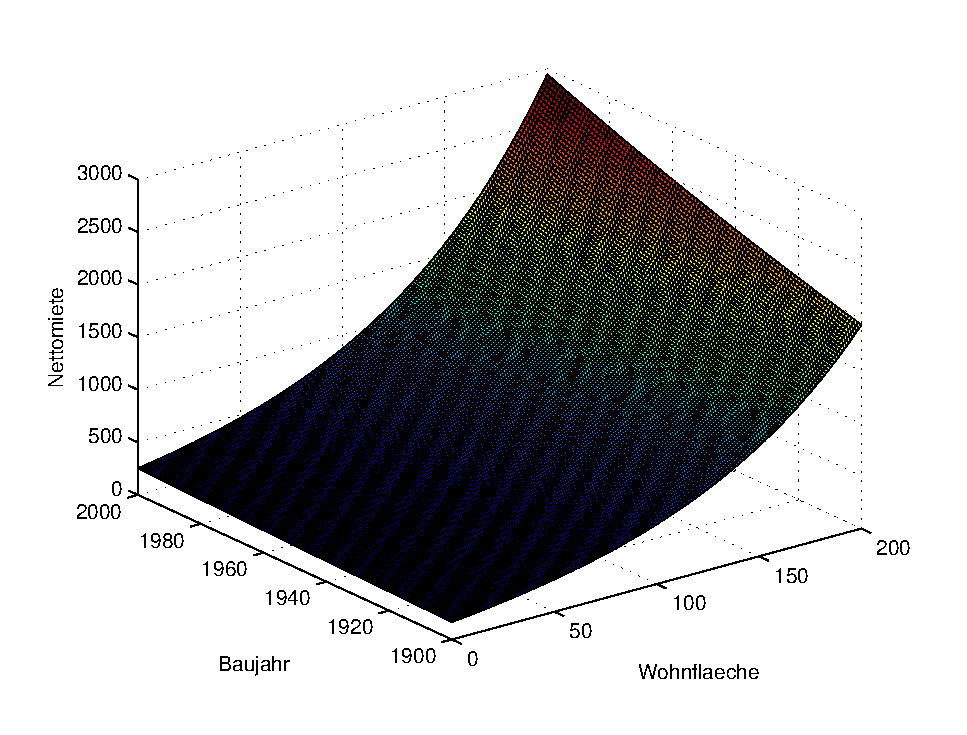
\includegraphics[width=10cm]{figures/nm_wfl_bj_log_approach}
  \caption{Caption}
  \label{fig:3d_result}
\end{figure}




%\subsection{Analyse}

%TODO:Überarbeiten oder herausnehmen!
%Zusätzlich zu der Berechnung der verschieden Regressionsmodelle bietet die {\it NAG C Library} auch Funktionen zur Auswahl des Regressionsmodells und zur Modellvalidierung.

%Für die Auswahl des Modells sollen in der Arbeit zwei Metriken behandelt werden: Die Residualstreuung und das Bestimmtheitsmaß $\mathcal{R}^2$.
%Beide können uns eine Idee davon geben, wie gut die unabhängigen Variablen die Werte der abhängigen Variablen erklären können.
%Die Residualstreuung gibt die Verteilung der Differenzen zwischen der angenäherten Funktion und den wirklichen Daten an.
%Sollte sie unregelmäßig sein (wenn die Residuen beispielsweise mit einer Variablen anwachsen) ist dies ein starkes Indiz dafür, dass ein zu simples Modell gewählt wurde. 
%Das Bestimmtheitsmaß gibt dagegen an, wie gut abhängige Variable durch die Regression erklärt werden kann.
%Berechnet werden kann es auch durch eine Quadrierung des Bravais-Pearson Korrelationskoeffizienten, was den starken Zusammenhang von Korrelation und Regressionsanalyse zeigt.

%Für die Modellvalidierung stehen verschiedene Werkzeuge zur Verfügung, welche bei der Bewertung der Güte der Regression und deren Verbesserung genutzt werden können.
%In diese Kategorie fallen zum Beispiel der Cooks-Abstand (ermittelt besonders einflußreiche Punkte), die T-Statistik (Testet, ob eine unabhängige Variable für die Regression wichtig ist) oder der Durbin-Watson-Test (Ermittelt, ob die Residuen von den zuvor gemessenen Werten abhängig sind.
%In dieser Arbeit werden diese allerdings nicht weiter behandelt werden.

%%% Local Variables: 
%%% mode: latex
%%% TeX-master: "report"
%%% End: 
